\documentclass[10pt]{article}

\usepackage[accepted]{rlc}
% If accepted, instead use the following line for the camera-ready submission:
%\usepackage[accepted]{rlc}
% To de-anonymize and remove mentions to RLC (for example, for posting to preprint servers), instead use the following:
% \usepackage[preprint]{rlc}

\usepackage{array}
\usepackage{amsmath}
\usepackage{amsthm}
\usepackage{amsbsy}
\usepackage{amssymb}
\newtheorem{definition}{Definition}
\usepackage{graphicx}
\usepackage{mathtools}
\usepackage{nicefrac}
\usepackage{bm}
\usepackage{enumitem}
\usepackage{mpemath}
\usepackage{tcolorbox}
\usepackage[capitalize,noabbrev]{cleveref}
\usepackage{theoremref}
\usepackage{thmtools}
\usepackage{thm-restate}
\usepackage{algorithm}
\usepackage{algpseudocode}
\usepackage{tikz}
\usepackage{subcaption}
\usepackage{hyperref}
\usepackage{dsfont}
\usepackage{bbm}


\bibliographystyle{abbrvnat}
\usepackage[framemethod=default]{mdframed}

\renewcommand{\cite}{\citep}

\renewcommand{\algorithmicrequire}{\textbf{Input:}}
\renewcommand{\algorithmicensure}{\textbf{Output:}}
\newcommand{\cvar}{\text{CVaR}}
\newcommand{\cvaralpha}{\text{CVaR}_\alpha}
\newcommand{\var}{\text{VaR}}
\newcommand{\varalpha}{\text{VaR}_\alpha}


\theoremstyle{plain}
\newtheorem{theorem}{Theorem}
\newtheorem{lemma}{Lemma} 
\newtheorem{proposition}{Proposition}
\newtheorem{assumption}{Assumption}
\theoremstyle{remark}
\newtheorem{example}{Example}

% \newcommand{\mm}[1]{\textcolor{magenta}{[#1]}}
% \newcommand{\db}[1]{\textcolor{blue}{[DB: #1]}}
% \newcommand{\gersi}[1]{\textcolor{red}{[#1]}}
% \newcommand{\s}[1]{\mathcal{#1}}

\DeclareMathOperator{\ext}{ext}

% \setlength{\parskip}{3mm plus 1mm minus 1mm}
% \setlength{\parindent}{0pt}

\title{Survey on Risk-Averse Reinforcement Learning}
\author{Gersi Doko \\
        Gersi.Doko@unh.edu \\}


\begin{document}

\maketitle

\section{Introduction}

Reinforcement learning (RL) is a powerful framework for developing agents that can learn to make decisions in complex, uncertain environments.
The core goal of RL is to tractably compute an optimal policy for acting in such an environment. A key challenge in RL is 
that the environment is often stochastic, and the agent may have only partial observability. 
Choosing an objective function that accurately captures the desired behavior of the agent is a difficult task.

We would hope the objective that an RL agent aims to optimize would consider the "risk" of the actions it takes.
One first needs to consider how to quantify risk into a numerical value. A value that encapsulates the uncertainty of the outcome of an action,
so that an agent can distinguish between actions that are risky and those that are safe.

There is a vast field of research that focuses on developing risk measures.
The goal of a risk measure is to quantify the uncertainty of a random variable, often while being interpretable and computationally tractable.
The intersections of risk and reinforcement learning is the topic of this review, where we will explore the field of risk-averse reinforcement learning.

\section{Preliminaries}

In order to introduce the concepts of risk-averse reinforcement learning, we first need to define some basic concepts in probability theory and reinforcement learning.

We adopt the common notation that $\Delta^n$ denotes the $n$-dimensional simplex. For two sets $A$ and $B$, $A^B$ denotes the set of all functions from $B$ to $A$.
For a set $A$, $|A|$ denotes the cardinality of $A$[].

The enviornment is a Markov Decision Process (MDP) defined by a tuple $\mathcal{M} = (\mathcal{S}, \mathcal{A}, \mathcal{P}, r, \gamma)$ where
\begin{itemize}
        \item $\mathcal{S}$ is the state space,
        \item $\mathcal{A}$ is the action space,
        \item $\mathcal{P} : \mathcal{S} \times \mathcal{A} \to \Delta^\mathcal{S}$ is the transition probability function,
        \item $r : \mathcal{S} \times \mathcal{A} \to \Real$ is the reward function,
        \item $\gamma \in [0, 1$ is the discount factor.
\end{itemize} 
Finally, we define the set of all deterministic policies $\Pi_D = \mathcal{A}^\mathcal{S}$. 
And the set of all randomized policies $\Pi_R = [\Delta^\mathcal{A}]^\mathcal{S}$.
We encourage the reader to refer to~\cite{Puterman1994} for a more detailed introduction to MDPs.

\section{Risk and Reward}

\begin{definition}[Risk Measure]
        \label{def:risk}
        A Risk Measure is a mapping from a random variable to a real number. Quantifying the uncertainty of an outcome.
        Given a metric space ($\Omega$, $\mathcal{F}$, $P$), a risk measure is a function $\psi: \mathcal{X} \to \Real$. Satisfying
        \begin{enumerate}
                \item Monotonicity: $X \leq Y \implies \psi(X) \leq \psi(Y)$
                \item Translation Invariance: $\psi(X + c) = \psi(X) + c \quad \forall c \in \Real$
        \end{enumerate}
\end{definition}

\begin{definition}[Variance]
        \label{def:variance}
        The variance of a random variable $X$ is defined as 
        $$\text{Var}(X) = \mathbb{E}[(X - \mathbb{E}[X])^2].$$
\end{definition}

\begin{definition}[Expectation]
        \label{def:expectation}
        A common risk measure is the expectation of a random variable. Given a random variable $X: \Omega \to \Real$, the expectation of $X$ is defined as
        $$\mathbb{E}[X] = \sum_{\omega \in \Omega} X(\omega) P(\omega).$$
\end{definition}

\begin{definition}[Value at Risk (Var)]
        The Value-at-Risk (VaR) of a random variable $X$ at risk-level $\alpha$ is defined as
        $$\varalpha(X) = \inf \left\{ t \in \Real \mid P(X \leq t) \geq \alpha \right\}.$$
\end{definition}

\begin{definition}[Conditional Value-at-Risk (CVaR)]
        \label{def:cvar}
        The Conditional Value-at-Risk (CVaR) of a random variable $X$ at risk-level $\alpha$ is defined as
        $$\cvaralpha(X) = \min_{t \in \Real} \left\{ t + \frac{1}{1 - \alpha} \mathbb{E}[(X - t)_+] \right\}.$$
\end{definition}


\begin{figure}[ht!]
        \begin{subfigure}[t]{0.5\textwidth}
                \centering
                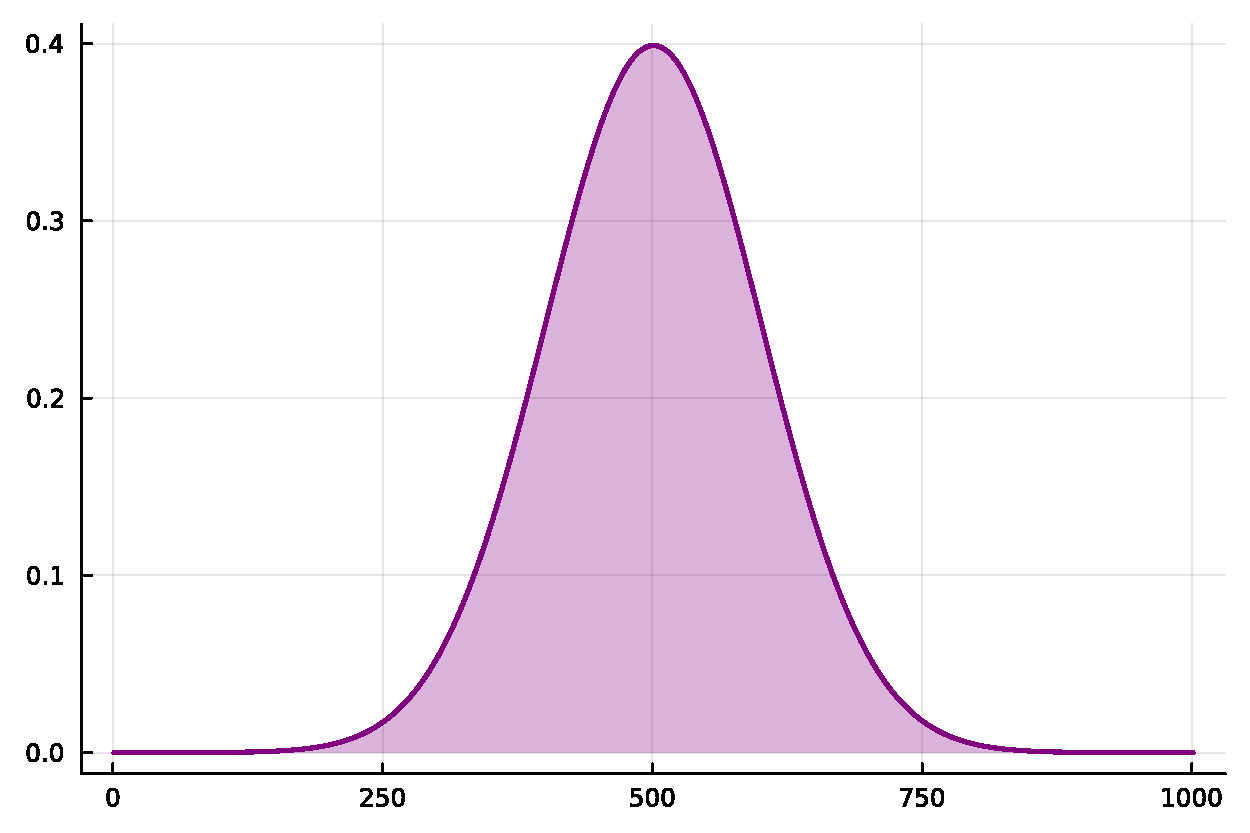
\includegraphics[width=0.7\linewidth]{julia_figures/normal.pdf}
                \caption{$\mathcal{N}(0,1)$}
                \label{fig:normal}
        \end{subfigure}
        \begin{subfigure}[t]{0.5\textwidth}
                \centering
                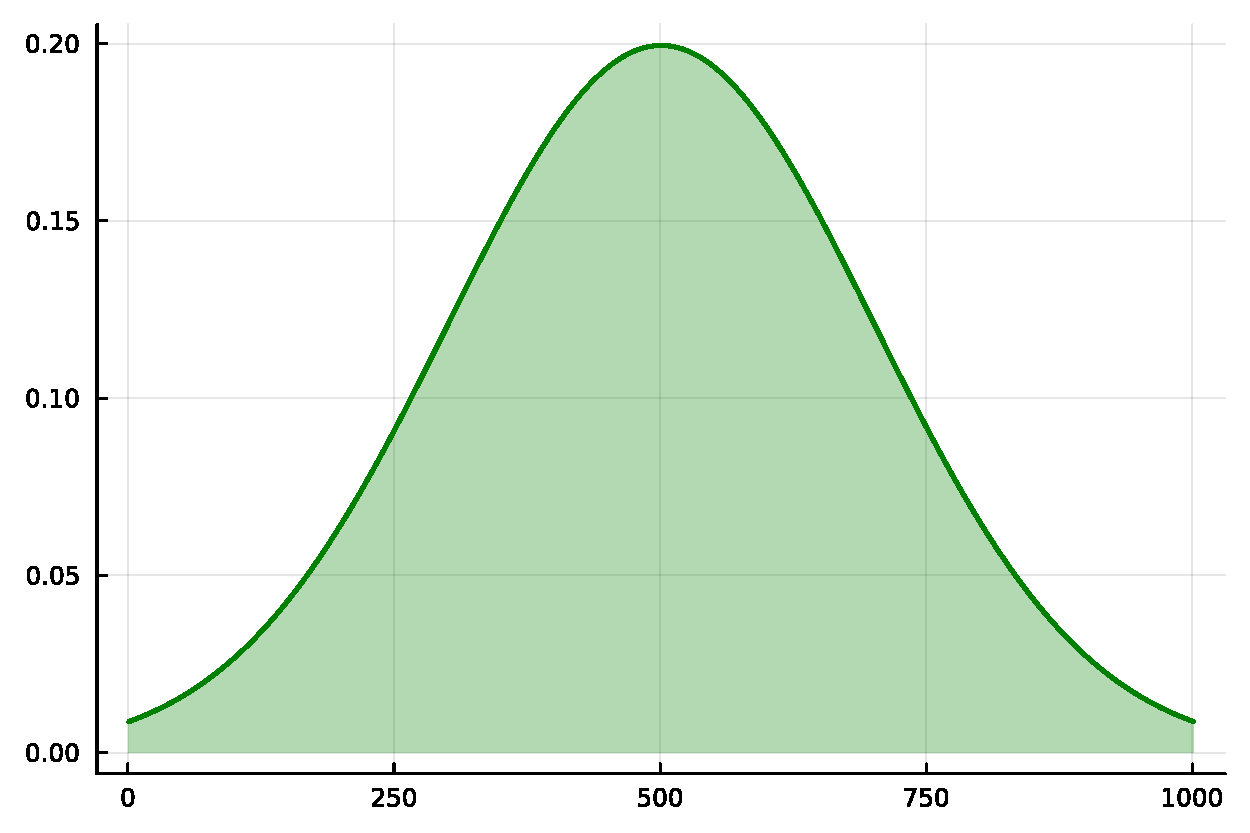
\includegraphics[width=0.7\linewidth]{julia_figures/normal_wide.pdf}
                \caption{$\mathcal{N}(0,2)$}
                \label{fig:normal_wide}
        \end{subfigure}
        \begin{subfigure}[t]{1.0\textwidth}
                \centering
                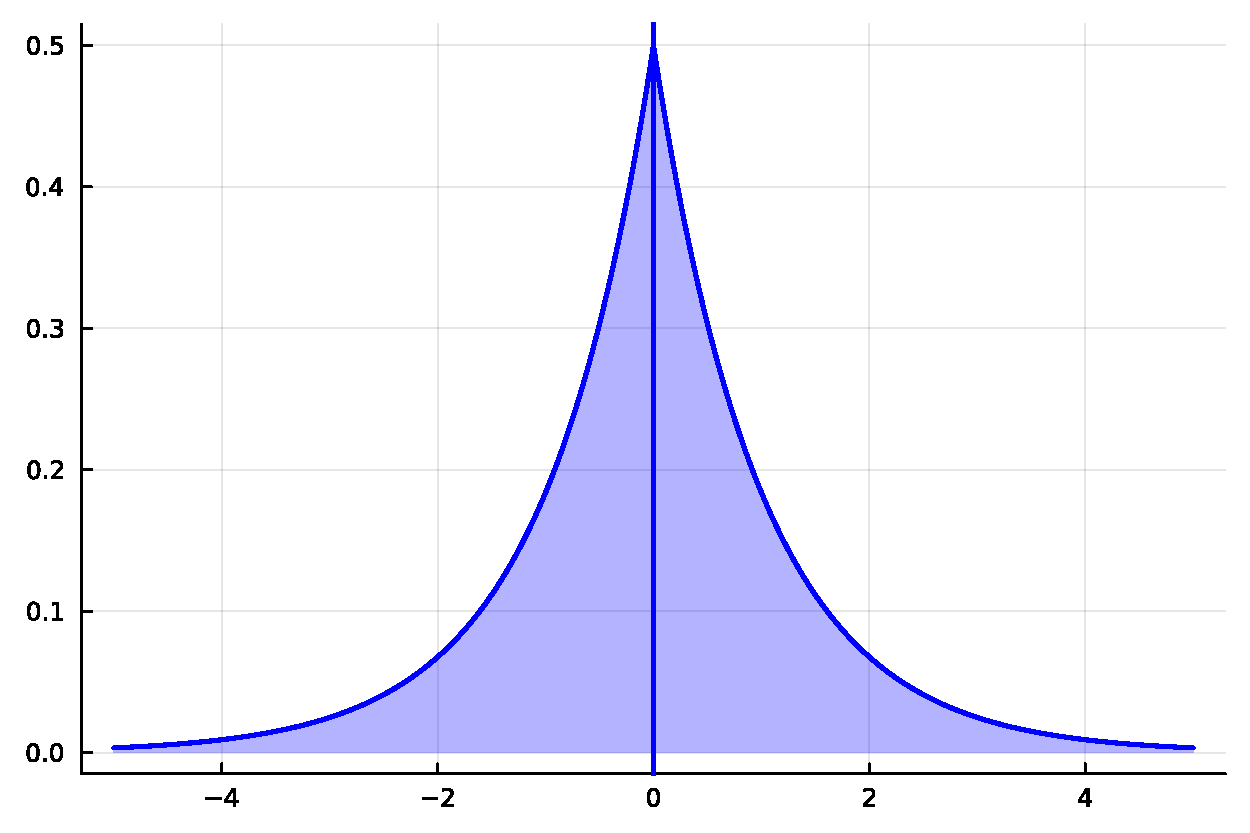
\includegraphics[width=0.4\linewidth]{julia_figures/laplace.pdf}

                \caption{$\mathcal{L}(0,1)$}
                \label{fig:laplace}
        \end{subfigure}
        \caption{Probability Density Functions of Various Distributions. All with a shared mean of 0.}
        \label{fig:pdfs}
\end{figure}

\section{Vanilla Reinforcement Learning}

In order to make decisions one must adopt a policy which prescribes the agent's behavior.
A policy is a mapping from states to actions, and the goal of reinforcement learning is to find an optimal policy that maximizes the expected return.
Policies may depend on time, and the agent may have a horizon of $T$ time steps to act. 
In this paper we assume a finite horizon, with each $s \in S$ having a time component, thus we omit the subscript $t$ on all variables for simplicity.

\begin{definition}[Finite Horizon Expected Return]
        Given a policy $\pi : \mathcal{S} \to \Delta^\mathcal{A}$ the expected finite horizon discounted return $\rho(\pi)$ can be defined as
        $$\rho(\pi) = \mathbb{E}_{\pi, \mathcal{P}} \left[ \sum_{t=0}^{T} \gamma^t r(s_t, \pi(s_t)) \right].$$
        Where $s_0 \sim p_0$ and $s_{t+1} \sim \mathcal{P}(s_t, \pi(s_t))$, $\gamma$ is the discount factor, and $T$ is the time horizon.
\end{definition}

\begin{definition}[Objective of Reinforcement Learning]
        \label{def:rl_obj}
        The objective of reinforcement learning (RL) is as follows
        $$\max_{\pi \in \Pi} \rho(\pi).$$
\end{definition}

\begin{definition}[Optimal Policy]
        \label{def:optimal_policy}
        An optimal policy $\pi^* \in \argmax_{\pi \in \Pi} \rho(\pi)$.
\end{definition}

Notice in \ref{def:optimal_policy} that the optimal policy may not be unique, 
as there may be multiple policies that achieve the same expected return. 
In practice, other methods such as entropy are used to score policies that are otherwise equivalent for interpretability.


\section{Risk-Averse Reinforcement Learning}

\section{Methods}

\bibliography{main.bib}

\end{document}
